%%%%%%%%%%%%%%%%%%%%%%%%%%%%%%%%%%%%%%%%%%%%%%%%%%%%%%%%%%%%%%%%
% Sablona pro zaverecnou zpravu k semestralni praci z BI-ZUM
% Kódování dokumentu: UTF8
% Verze: 1.0 (2013-01-28)
% Autor: Ing. Martin Šlapák
%%%%%%%%%%%%%%%%%%%%%%%%%%%%%%%%%%%%%%%%%%%%%%%%%%%%%%%%%%%%%%%%
%
% NEUPRAVUJTE PROSIM PARAMETRY DOKUMENTU, JAKO OKRAJE CI PISMO!
%
%%%%%%%%%%%%%%%%%%%%%%%%%%%%%%%%%%%%%%%%%%%%%%%%%%%%%%%%%%%%%%%%
%
% Celkova delka zpravy nesmi presahnout 1 stranu A4, vyjadrujte 
% se strucne, jasne a vecne - zadne omacky a slovni vata. Diky!
% Neprehazujte ani poradi sekci.
%
%%%%%%%%%%%%%%%%%%%%%%%%%%%%%%%%%%%%%%%%%%%%%%%%%%%%%%%%%%%%%%%%
\documentclass[a4paper,10pt,twocolumn]{article}
\usepackage{lmodern}
\usepackage[czech]{babel}
\usepackage[T1]{fontenc}
\usepackage[utf8]{inputenc}
\usepackage{graphicx}
\usepackage{float}
\usepackage[top=0.5cm,bottom=2cm,left=1cm,right=1cm]{geometry}
%gobble sezere cisla stranek, takze nebudou zadna
\pagenumbering{gobble} 
\title{Zpráva k 2. domácímu úkolu z předmětu MI-PAA}
\date{\today}
%%%%%%%%%%%%%%%%%%%%%%%%%%%%%%%%%%%%%%%%%%%%%%%%%%%%%%%%%%%%%%%%
% tady nastavte své jméno a email
\author{Jan Sokol \\ sokolja2@fit.cvut.cz}
%%%%%%%%%%%%%%%%%%%%%%%%%%%%%%%%%%%%%%%%%%%%%%%%%%%%%%%%%%%%%%%%
\begin{document}
\maketitle
%%%%%%%%%%%%%%%%%%%%%%%%%%%%%%%%%%%%%%%%%%%%%%%%%%%%%%%%%%%%%%%%
\begin{abstract}
Úkolem bylo nalézt řešení 0/1 problému batohu hrubou silou (tj. nalezení skutečného optima). Dále bylo třeba zkušebních datech pozorovat závislost výpočetního času na n (kde n je počet věcí v batohu). Druhou částí ukolu naprogramování řešení problému batohu dalšími, pokročilými metodami.
 \begin{itemize}
\item První byla metoda větví a hranic (B\&B). A to tak, aby omezujícím faktorem byla hodnota optimalizačního kritéria. Tj. při ořezávání shora omezení bylo překročení kapacity batohu. Omezení zdola bylo řešeno podmínkou, že stávající řešení nemůže být lepší než nejlepší dosud nalezené. Tato metoda je lepší (rychlejší) prořezávání prostorem, než je hrubá síla,
\item metodou dynamického programování,
\item FPTAS algoritmem, (tj. s použitím modifikovaného dynamického programování s dekompozicí podle ceny).

\end{itemize} 
Na těchto datech bylo třeba pozorovat závislost výpočetního času na n (a to také s metodami z minulé úlohy - hrubou silou a jednoduchou heuristikou).




% Zde shrňte v několika větách co jste dělali, jak jste to dělali, jakých výsledků jste dosáhli. Vypíchněte to nejzajímavější. Zkusili jste nějakou pokročilou techniku? Tady se s ní pochlubte a pak ji dále rozepište v patřičné sekci. Zkuste se vejít do 150 slov.
\end{abstract}

%%%%%%%%%%%%%%%%%%%%%%%%%%%%%%%%%%%%%%%%%%%%%%%%%%%%%%%%%%%%%%%%
\section{Výběr jazyka, popis implementovaných metod}
Pro svou implementaci problému batohu jsem si vybral jazyk Python. Ačkoli to je jazyk interpretovaný a nečekal jsem závratné rychlosti výpočtů, mojím výběrem byl pro to, že jsem jazyk znal a pro jakýkolik koncept je pro mne nejrychlejší.

V případě hledání řešení hroubou silou jsem těžil z materiálů v přednáškách, tak i na internetu.


Metoda branch and bound zajišťuje, že prostor je prořezáván jak zdola, tak shora. Ty větve v rekurzi, které by neposkytly lepší výsledek (či by přesáhny kapacitu batohu), nejsou dále procházeny. V paměti držen nejlepší výsledek (globální hodnota). Před každým sestoupením do spodní větve se zkontroluje cena zbývajíchích (ještě nepřidaných) předmětů. Pokud součet cen zbývajících itemů a držené ceny batohu je menší, než nejlepší výsledek, k lepší hodnotě už se není možné dostat a průchod ukončujeme.

Pomocí metody dynamického programování přesouváme náročnost na CPU na paměťovou náročnost. Vybral jsem dekompozici dle ceny - abych funkce dále mohl využít i pro metodu FPTAS. V paměti držíme tabulku (decomposition table), kam ukládáme mezivýpočty. Sloupce jsou ceny, řádky jsou předměty. Těmito mezivýpočty jsou aktuální váhy v batohu. Výsledek je poté možné vidět ve spodním řádku - ta hodnota, co je nejvíce napravo.

Při výpočtu FPTAS můžeme ovlivnit kvalitu výsledku tím, že nastavíme proměnnou accurancy. Tou je možné definovat maximální relativní chybu, se kterou algoritmus bude pracovat. Zde jde o zanedbání určitého počtu bitů z ceny. Ceny předmětů jsou zpoměrovány, a poté je výpočet stejný, jako u dynamického programování.


\section{Testovací Hardware}
Všechny testy byly prováděny na cloudové linuxové instanci v AWS, běžící na Red Hat Enterprise Linux 7. Velikost instance byla:
  2 Core CPU / 8 GB RAM, v názvosloví AWS \textbf{m4.large}.


\section{Měření výpočetního času}
Výpočet běhu funkce je řešen tak, že je spočten strojový čas před během funkce, a také po něm. Tyto časy jsou od sebe odečteny a je vrácen čas v ms.

   \begin{verbatim}
def timing(f):
    def wrap(*args):
        time1 = time.time()
        ret = f(*args)
        time2 = time.time()
        measured_time.append(
          {'type': f.__name__,
           'time': (time2-time1)*1000.0})
        return ret
    return wrap
   \end{verbatim}


\subsection{Výpočetní časy jednotlivych metod}

\begin{figure}[H]
  \begin{center}
    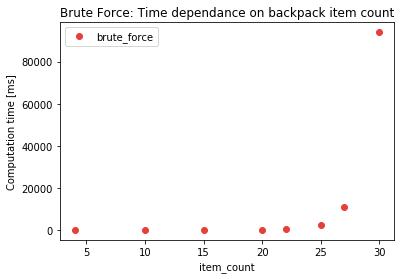
\includegraphics[height=6cm]{graphs/bruteforce_speed.png}
  \end{center}
  % \caption{Graf vývoje fitness}\label{fig1}
\end{figure}

\begin{figure}[H]
  \begin{center}
    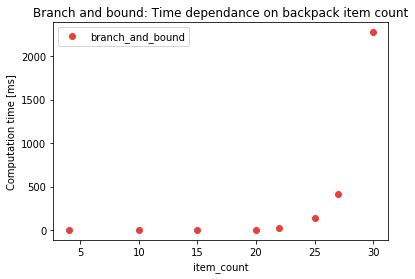
\includegraphics[height=6cm]{graphs/bnb_speed.png}
  \end{center}
  % \caption{Graf vývoje fitness}\label{fig1}
\end{figure}


\begin{figure}[H]
  \begin{center}
    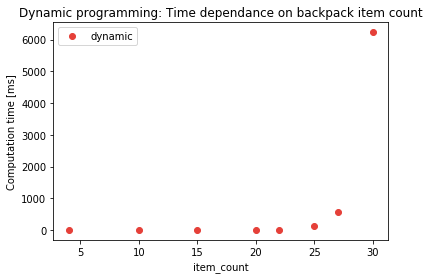
\includegraphics[height=6cm]{graphs/dynamic_speed.png}
  \end{center}
  % \caption{Graf vývoje fitness}\label{fig1}
\end{figure}


\begin{figure}[H]
  \begin{center}
    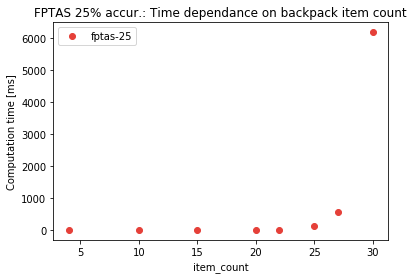
\includegraphics[height=6cm]{graphs/fptas25_speed.png}
  \end{center}
  % \caption{Graf vývoje fitness}\label{fig1}
\end{figure}



\subsection{Srovnání výpočetních časů}


Zde přikládám srovnání výpočetních časů hrubé síly, B\&B, dynamického programování a aproximativního algoritmu (FPTAS).

\begin{figure}[H]
  \begin{center}
    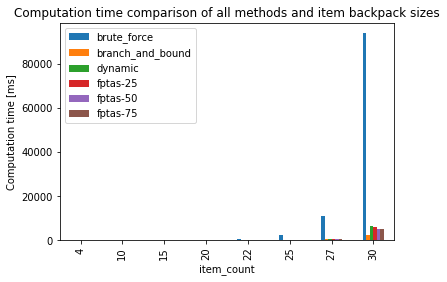
\includegraphics[height=6cm]{graphs/all_speed_comparison.png}
  \end{center}
  % \caption{Graf vývoje fitness}\label{fig1}
\end{figure}

\begin{figure}[H]
  \begin{center}
    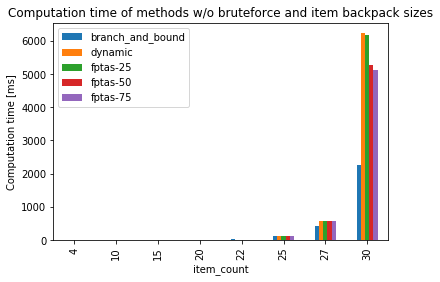
\includegraphics[height=6cm]{graphs/no_brute_speed_all.png}
  \end{center}
  % \caption{Graf vývoje fitness}\label{fig1}
\end{figure}



\subsection{FPTAS - závislost chyby a výpočetního času algoritmu na přesnosti zobrazení}

...


\begin{figure}[H]
  \begin{center}
    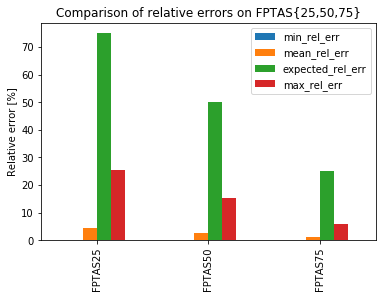
\includegraphics[height=6cm]{graphs/fptas_err_all.png}
  \end{center}
  % \caption{Graf vývoje fitness}\label{fig1}
\end{figure}



\section{Shrnutí a výsledky}

Pomocí metody hrubé síly jsem dosáhl pouze velikosti 27 - při velikosti bahohu již vypočtení testovacích dat trvalo více než 24 hodin. Díky tomu v grafech větší data pro měření rychlostí nejsou přiložena. 
Relativní chyba používá data z referenčního řešení, a díky tomu, že řešení heuristikou je mnohem rychlejší, než hrubou silou, proto data obsahuje pro všechny zadaná data.

Pro vytváření grafů bylo využito Python notebooku, který je přiložen v adresáři \textbf{report/}. Grafy jsou vykresleny pomocí knihovny \textbf{mathplotlib}.

% Tady okomentujte k čemu se váš evoluční algoritmus dopracoval, co se vám povedlo, co ne a jak by to šlo vylepšit. Jakého nejlepšího řešení se vám podařilo dosáhnout. Klidně i napište, co se vám na semestrální práci líbilo a taky co byste raději měli jinak. Uvítáme jakékoli nápady. 

% Pokud jste čerpali z nějaké literatury, měli byste ji řádně ocitovat.

% \textbf{A NEZAPOMEŇTE, ŽE SE MUSÍTE VEJÍT NA JEDNU A4! ;-)}

%%%%%%%%%%%%%%%%%%%%%%%%%%%%%%%%%%%%%%%%%%%%%%%%%%%%%%%%%%%%%%%%
% odtud dal to pak zakomentujte pomoci znaku procenta na zacatku radku
% \begin{center}
% \line(1,0){250}
% \end{center}

% \textbf{Pár poznámek pod čarou\ldots}
% \begin{itemize}
%   \item Zdroják této šablony je v kódování UTF8.
%   \item Neměňte prosím žádná nastavení dokumentu, okrajů, velikosti písma apod.
%   \item Nepřehazujte ani pořadí sekcí.
%   \item \textbf{Jak zprávu zkompilovat?} Použijte dvakrát (kvůli odkazům a referencím) tento příkaz:

%   \begin{verbatim}
%   pdflatex zdrojak-zpravy.tex
%   \end{verbatim}

%   Výsledkem bude \textbf{zdrojak-zpravy.pdf}. 

%   \item Pokud něco nepůjde, konzultujte na cvičeních BI-TED či se spolužáky. Cvičící BI-ZUM nebudou mít čas řešit detaily s {\LaTeX}em.
%   \item \textbf{Proč se sakra musím vejít na 1 A4?} Chceme, abyste si vyzkoušeli jak napsat to podstatné, vybrat to důležité, vyhnout se takové té textové vatě. Současně po vás nechceme psaní dlouhých esejí, raději svůj čas věnujte svým algoritmům. A taky, kdo má číst 5 stran napsaných \uv{protože to chtěj}. ;-)
%   \item TIP: Tuto zprávu může být reálné uplatnit i jako jeden z domácích úkolů na BI-TED. K tomu vás ale nenutíme a také počítejte s tím, že tam po vás mohou chtít další rozšíření dokumentu. \textbf{Ale zase: proč nezabít dvě mouchy jednou ranou?}
% \end{itemize}

\end{document}
